\beginsong{Lang war die Reise}[txt={Jörg Ermisch, 1990}, mel={aus Irland}, bo={226}, pfii={109}, pfiii={60}]

\beginverse
\endverse
\centering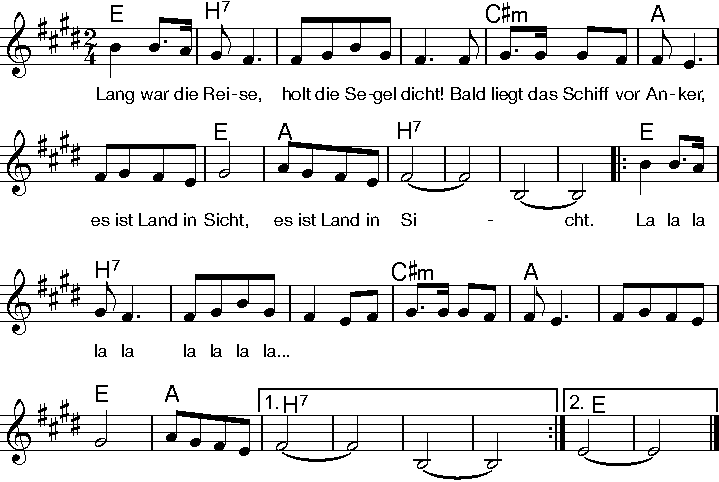
\includegraphics[width=1\textwidth]{Noten/Lied061.pdf}	

\beginverse
\[E]Wie oft sah \[H7]ich im Nebel die Hand vor Augen nicht?
Bald \[C#m]klärt sich der \[A]Himmel, 
es ist Land in \[E]Sicht, \[A]es ist Land in \[H7]Sicht.
\endverse

\beginchorus
\lrep \[E]La la \[H7]la la \[C#m]la la la la \[A]la la \[E]la la \[A]la la la la la la \[H7]la la la la \rrep
\endchorus

\beginverse
^Zwei blaue ^Augen waren voller Licht.
Die ^Fahrt geht immer ^weiter, 
es ist Land in ^Sicht, ^es ist Land in ^Sicht.
\endverse

\renewcommand{\everychorus}{\textnote{\bf Refrain (wdh.)}}
\beginchorus
\endchorus

\beginverse
^Seht, wie die ^Sonne durch den Nebel bricht!
Ein ^Meer voller ^Blumen, 
es ist Land in ^Sicht, ^es ist Land in ^Sicht. 
\endverse

\beginchorus
\endchorus

\beginverse
^Wer weiß, ob schon ^morgen eine neue Zeit anbricht?
Die ^Fahrt geht immer ^weiter,
es ist Land in ^Sicht, ^es ist Land in ^Sicht.
\endverse

\beginchorus
\endchorus

\endsong

\begin{intersong}
\ifthenelse{\boolean{pics}}{
    \ThisLRCornerWallPaper{1}{Bilder/langwardiereise.png}
}{}
\end{intersong}